\chapter{Die Realisierung}
\label{cha:Realisierung}
Dieses Kapitel befasst sich mit der Implementierung der Spezifikation des Vorlagenmanagements, die im Kapitel \ref{cha:Lösungskonzept} vorgestellt wurde. Die Implementierung wurde in \emph{Java 8} mit dem \emph{Buildtool-Maven} realisiert, wobei die Implementierungen in der folgenden Projektstruktur organisiert wurden.
\begin{figure}[h]
\dirtree{%
.1 mailing.
.2 model.
.3 jpa.
.2 module.
.3 template.
.4 cdi.
.4 jsf.
.4 model.
.5 json.
.4 logic.
.5 api.
.5 impl.
.3 integration.
.4 clevercure-web.
.2 testsuite.
.3 cdi.
.2 demo.
.3 logic.
.3 web.
.2 data.
.3 api.
.3 impl.
}
\caption{Verzeichnisstruktur der \emph{Maven}-Projekte}
\label{fig:minimal-example:frame-dirtree}
\end{figure}
\ \newline
Das \emph{Maven}-Wurzelprojekt \emph{mailing} organisiert die Metadaten wie die EntwicklerInnen, die an diesem Projekt mitwirken, alle benötigten Abhängigkeiten, sowie die auf alle Unterprojekte anwendbare \emph{Build}-Konfigurationen. Die übergeordneten Projekte sind vom Typ \emph{pom}, was bedeutet, dass aus diesen Projekten keine Artefakte erstellt werden und die übergeordneten Projekte die tiefer liegenden Projekte bündeln. Die gesamte Organisation der Abhängigkeiten findet im Wurzelprojekt \emph{mailing} statt. Diese Projektstruktur wurde gewählt, da in diesem Projekt auch die Implementierungen der anderen Softwarekomponenten von \emph{CleverMail} organisiert werden. Die konkreten Artefakte wurden jeweils in ein Artefakt \emph{*-api} und \emph{*-impl} aufgeteilt, somit sind die Schnittstellen (Spezifikationen) vollständig getrennt von deren Implementierungen. Folgende Auflistung beschreibt alle konkreten Artefakte \emph{(Java-Archive)}, die aus dem Wurzelprojekt \emph{mailing} erstellt werden können:
\begin{itemize}
	\item\emph{\textbf{mailing-model-jpa}} 
	\newline
	ist das Artefakt, das die Klassen mit den \emph{JPA-}-Entitäten enthält, die die Datenbank in \emph{Java} abbilden.
	\item\emph{\textbf{mailing-module-template-cdi}} 
	\newline
	ist das Artefakt, das die Implementierung der \emph{CDI}-Erweiterung für die Integration in eine \emph{CDI}-Umgebung  enthält.
	\item\emph{\textbf{mailing-module-template-jsf}}
	\newline
	ist das Artefakt, das die Implementierung für die Integration in \emph{JSF} enthält.
	\item\emph{\textbf{mailing-module-template-model-json}}
	\newline
	ist das Artefakt, das die Implementierung der \emph{JSON}-Datenobjekte in Form von \emph{Java}-Klassen enthält.	
	\item\emph{\textbf{mailing-module-template-logic-api}} 
	\newline
	ist das Artefakt, das die Spezifikation des Vorlagenmanagements enthält.
	\item\emph{\textbf{mailing-module-template-logic-impl}} 
	\newline
	ist das Artefakt, das die Implementierung der Spezifikation des Vorlagenmanagements enthält.
	\item\emph{\textbf{mailing-module-integartion-clevercure-web}}
	\newline
	ist das Artefakt, das die Implementierung der Integration für die Anwendung \emph{CleverWeb} enthält.
	\item\emph{\textbf{mailing-testsuite-cdi}},
	\newline
	ist das Artefakt, das die Ressourcen aller Tests, die in einer \emph{CDI}-Umgebung lauffähig sein müssen, enthält.
	\item\emph{\textbf{mailing-demo-logic}}
	\newline
	ist das Artefakt, das die Schicht der Geschäftslogik der Beispielanwendung enthält.
	\item\emph{\textbf{mailing-demo-web}}
	\newline
	ist das Artefakt, das die \emph{Web}-Anwendung der Beispielanwendung enthält.
	\item\emph{\textbf{mailing-data-api}}
	\newline
	ist das Artefakt, dass die Spezifikation der Geschäftslogik enthält, die die Persistenz der \emph{E-Mail}-Vorlagen behandeln. Es enthält auch die Datenbankzugriffsklassen in Form von \emph{Data-Repository}-Schnittstellen.
	\item\emph{\textbf{mailing-data-impl}}
	\newline
	ist das Artefakt, das die Implementierung der Geschäftslogik enthält.
\end{itemize} 

\section{Die Implementierung der Spezifikationen}
Dieser Abschnitt behandelt die Implementierungen der Spezifikationen, die im Kapitel \ref{cha:Lösungskonzept} vorgestellt wurden. 

\subsection{Die Implementierung für \emph{CKEditor}}
Wie im Abschnitt \ref{sec:sub-typescript-javascript} vorgegeben, wurde ein \emph{Plugin} in \emph{TypeScript} implementiert, dass innerhalb des \emph{CKEDitors} die Variablen verwaltet. Die Implementierung des \emph{Plugins} in \emph{TypeScript} war möglich, da für den \emph{Editor CKEditor} vom dem, von \emph{Microsoft} verwalteten, \emph{Open-Source} Projekt \emph{DefinitelyTyped} Typinformationen für \emph{TypeScript} bereitgestellt werden, die die \emph{JavaScript}-Schnittstellen als \emph{TypeScript}-Schnittstellen definieren. Hätten keine Typinformationen zur Verfügung gestanden, hätte man die Typinformationen selber implementieren müssen, was einen erheblichen Mehraufwand bedeutet hätte.
 
\subsubsection{Das \emph{CKEditor-Plugin} in \emph{Typescript}}
Das Variablenmanagement ist unabhängig vom verwendeten \emph{Editor} und wurde daher vom \emph{CKEditor-Plugin} logisch und physisch getrennt, wobei das Variablenmanagement im \emph{TypeScript}-Modul \emph{cc.variables} und das \emph{CKEDitor-Plugin} im \emph{TypeScript}-Modul \emph{cc.ckeditor.plugins} implementiert wurden. Die voneinander getrennten \emph{TypeScript}-Quelltextdateien werden beim Kompilieren in eine einzige \emph{JavaScript}-Quelltextdatei zusammengeführt. Mit der Organisation in eigenen \emph{TypeScript}-Modulen wird sichergestellt, dass nur explizit nach außen sichtbar gemachte \emph{(export MyType \{...\})} Funktionen oder Typen außerhalb des Moduls referenziert werden können. Ein \emph{TypeScript}-Modul wird in ein korrespondierendes \emph{JavaScript}-Modul übersetzt. Die Verwendung von Modulen bring auch den Vorteil, dass am \emph{Window}-Objekt nur das Objekt der Wurzel des Namensraums \emph{cc} gebunden ist, wodurch das \emph{Window}-Objekt nicht mit den eigenen\emph{JavaScript}-Objekten verschmutzt wird. Die Quelltexte aus den Abbildungen \ref{prog:example-typescript-modul} und \ref{prog:example-javascript-modul} zeigen ein \emph{TypeScipt}-Modul und das daraus resultierende \emph{JavaScript}-Modul.
\newpage

\begin{program}[h]
\caption{Das \emph{TypeScript}-Modul}
\label{prog:example-typescript-modul}
\begin{JsCode}[numbers=none]
module cc.ckeditor.plugins {
	export module variables {
		export interface VariableMapping{
	        id:string
		}
	}
}                  
\end{JsCode}
\end{program}

\begin{program}[h]
\caption{Das \emph{JavaScript}-Modul}
\label{prog:example-javascript-modul}
\begin{JsCode}[numbers=none]
var cc;
(function (cc) {
    var variables;
    (function (variables_1) {
    // VariableMapping nicht Teil des generierten JavaScripts
    })(variables = cc.variables || (cc.variables = {}));
})(cc || (cc = {}));                 
\end{JsCode}
\end{program}
\ \newline
Die \emph{TypeScript}-Schnittstelle \emph{VariableMapping} aus dem Quelltext aus Abbildung \ref{prog:example-typescript-modul} ist nicht Teil des generierten \emph{JavaScript}-Moduls, da diese Schnittstelle nur eine Typinformation für \emph{TypeScript} darstellt. Wäre die Schnittstelle \emph{VariableMapping} eine \emph{TypeScript}-Klasse, dann wäre diese Klasse auch Teil des generierten \emph{JavaScript}-Moduls und würde als \emph{JavaScript}-Funktion abgebildet werden.
\newline
\newline
Das Variablenmanagement in \emph{TypeScript} ist verantwortlich für die \emph{Browser}-seitige Registrierung der Variablen und stellt Hilfsmethoden zur Verfügung, mit denen Variablen in der \emph{HTML}-Vorlage gefunden und konvertiert werden können. Der Quelltext aus Abbildung \ref{prog:example-typescript-convert-variable} zeigt mehrere Möglichkeiten, wie eine Variable in \emph{TypeScript} konvertiert werden kann.
\newpage

\begin{program}[h]
\caption{Beispiele für Variablenkonvertierungen in \emph{TypeScript}}
\label{prog:example-typescript-convert-variable}
\begin{JsCode}
// Hilfsklasse für die Konvertierung der Variablen
class VariableUtils {
    private variables:VariableMapping[] = [];
	
    // Öffentliche Funktion für die Konvertierung der Variablen
    public convert(converter:(item:VariableMapping) => any 
    	                    = (item:VariableMapping)=> item):any[] {
        var converted:any[] = [];
        for (var i = 0; i < this.variables.length; i++) {
            converted[i] = converter(this.variables[i]);
        }
        return converted;	            
    }
}

// Eigene Klasse für die Konvertierung
class MyConverter {
    // Öffentliche Funktion für die Konvertierung der Variablen
    public convert(v:VariableMapping): any {
        return v.displayName;
    }
}

// Erstellen der Objekte aus den definierten Klassen
var util     :VariableUtils = new VariableUtils();
var converter:MyConverter   = new MyConverter();

// Konvertierung mit einer \emph{Arrow}-Funktion
util.convert((v:VariableMapping) => v.displayName);

// Konvertierung mit einer anonymen Funktion
util.convert(function (v:VariableMapping) {
    return v.displayName;
});

// Konvertierung mit einer Referenz auf eine Funktion
util.convert(converter.convert);
\end{JsCode} 
\end{program}
\ \newline
Die Funktion \emph{convert} der Klasse \emph{VariableUtil} aus dem Quelltext aus Abbildung \ref{prog:example-typescript-convert-variable} definiert den Formalparameter \emph{converter} als eine \emph{Arrow}-Funktion, die die Signatur der Funktion für die Konvertierung definiert und eine Standardimplementierung definiert, die verwendet wird, wenn bei der Aktivierung der Funktion \emph{convert} für den Formalparameter \emph{converter} kein Aktualparameter bereitgestellt wird.   Eine \emph{Arrow}-Funktion ähnelt einer \emph{Lambda}-Funktion in \emph{Java}. Der Typ \emph{any[]} ist vergleichbar mit dem Datentyp \emph{var} aus \emph{.NET} und gibt an, dass jeder Datentyp als Typ des zurückgelieferten \emph{Arrays} erlaubt ist.
\newpage

\subsubsection{Die Variablenrepräsentation in \emph{TypeScript}}
Die Variablen werden \emph{Java}-seitig als Objekte der Schnittstelle \emph{VariableContract} abgebildet, und müssen für das \emph{JavaScript}-seitige Variablenmanagement in eine \emph{JSON}-Zeichenkette überführt werden, die als \emph{JavaScript}-Objekte innerhalb von \emph{JavaScript} verwendet werden. Dafür wurde in \emph{TypeScript} die Schnittstelle \emph{VariableMapping} aus dem Quelltext aus Abbildung \ref{prog:example-typescript-variable-mapping} definiert, die die Struktur einer Variable innerhalb von \emph{TypeScript} definiert.
\begin{program}[h]
\caption{Die \emph{Typescript}-Schnittstelle \emph{VariableMapping}}
\label{prog:example-typescript-variable-mapping}
\begin{JsCode}
interface VariableMapping {    
    id:string,       
    displayName:string,        
    info:string
}
\end{JsCode}
\end{program}
\ \newline
Die Schnittstelle \emph{VariableMapping} ist Teil des Moduls \emph{cc.variables} und wird mit dem  \emph{TypeScript} Schlüsselwort \emph{export} nach außen offengelegt und kann über den vollständigen Pfad \emph{cc.variables.VariableMapping} innerhalb von \emph{TypeScript} referenziert werden. Mit der Schnittstelle \emph{VariableMapping} werden Typinformationen für die Variablenpräsentation in \emph{TypeScript} bereitgestellt, damit innerhalb von \emph{TypeScript} die Typsicherheit sichergestellt werden kann.

\subsubsection{Die Variablenrepräsentation in \emph{Java}}
Die Klasse \emph{VariableJson} aus dem Quelltext aus Abbildung \ref{prog:variableJson} zeigt die korrespondierende \emph{Java} Implementierung der Variablenrepräsentation. Mit der Klasse \emph{VariableJson} wird sichergestellt, das die Variablenrepräsentation in \emph{Java} korrespondierend zur Variablenrepräsentation in \emph{TypeScript} ist. Die Klasse \emph{VariableJson} stellt die Schnittstelle der Variablen definiert über die Schnittstelle \emph{VariableContract} zu \emph{TypeScript} bzw. \emph{JavaScript} dar. Als \emph{JSON-Provider} wird die Bibliothek \emph{FasterXML-Jackson-JSON}, vormals \emph{Jackson-JSON} genannt, verwendet, die es erlaubt mit Annotationen deklarativ Attribute und/oder Methoden einer Klasse auf \emph{JSON}-Attribute abzubilden. Durch den deklarativen Ansatz über Annotationen sind die annotierten  Attribute und/oder die annotierten Methoden einer Klasse entkoppelt von der Repräsentation in \emph{JSON} und können daher abgeändert werden ohne die Abbildung auf \emph{JSON} zu beeinflussen. Nur ein Ändern des Datentyps eines Attributes oder des Rückgabewerts einer Methode kann zu Problemen führen. 
\newline
\begin{program}
\caption{Die Schnittstelle \emph{VariableJson}}
\label{prog:variableJson}
\begin{JsCode}
@JsonTypeName(value = "variable-json")
public class VariableJson extends AbstractJsonModel {

    private String id;
    private String label;
    private String info;

    public VariableJson() {
    }

    public VariableJson(String id, 
                        String displayName, 
                        String tooltip) {
        this.id = id;
        this.label = displayName;
        this.info = tooltip;
    }

    @JsonGetter("id")
    public String getId() { 
        return id; 
    }

    @JsonSetter("id")
    public void setId(String id) { 
        this.id = id; 
    }

    @JsonGetter("displayName")
    public String getLabel() { 
        return label; 
    }

    @JsonSetter("displayName")
    public void setLabel(String label) { 
        this.label = label; 
    }

    @JsonGetter("info")
    public String getInfo() { 
        return info; 
    }

    @JsonSetter("info")
    public void setInfo(String info) { 
        this.info = info; 
    }
}
\end{JsCode}
\end{program}
\ \newline

\subsubsection{Registrierung des \emph{Plugins} im \emph{CKEditor}}
Das \emph{Plugin} wird über eine \emph{JavaScript}-Datei im \emph{CKEditor} registriert, wobei folgende Konventionen eingehalten werden müssen.
\begin{itemize}
	\item\emph{ckeditor/plugins}
	\newline
	ist das Verzeichnis, in dem das \emph{Plugin} enthalten sein muss.
	\item\emph{variables}
	\newline
	ist das Verzeichnis unterhalb des Verzeichnisses \emph{ckeditor/plugins}, in dem die \emph{Plugin}-Ressourcen enthalten sein müssen und das dem Namen des \emph{Plugins} entspricht.
	\item\emph{plugin.js}
	\newline
	ist die \emph{JavaScript}-Datei, die im Verzeichnis \emph{ckeditor/plugins/variables} liegen muss und das implementierte \emph{Plugin} darstellt. 
\end{itemize}
\ \newline
Der Quelltext aus Abbildung \ref{prog:example-ckeditor-config-js} zeigt einen Auszug aus der \emph{JavaScript}-Datei mit dem das \emph{Plugin} registriert wird und auch Einstellungen am \emph{CKEditor} vorgenommen werden können. Das \emph{Plguin} wird vom \emph{CKEditor} nach dessen Initialisierung geladen und registriert.

\begin{program}[h]
\caption{Registrierung des \emph{CKEditor-Plugins}}
\label{prog:example-ckeditor-config-js}
\begin{JsCode}
CKEDITOR.editorConfig = function (config) {
    config.extraPlugins = "variables";
}
\end{JsCode} 
\end{program}

\subsubsection{Integration des \emph{Plugins} im \emph{CKEditor}}
Die Abbildung \ref{fig:ckeditor-toolbar-opne-dialog} zeigt die Funktionsleiste des \emph{CKEditors}, in die der rot markierte \emph{Button} über das \emph{Plugin} eingefügt wurde. Durch einen Klick auf diesen \emph{Button} wird ein Dialog geöffnet, über den die zur Verfügung stehenden Variablen ausgewählt werden können.
\begin{figure}[h]
\centering
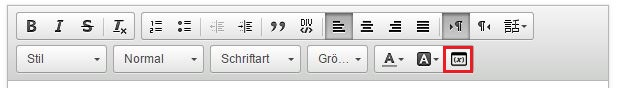
\includegraphics[scale=0.8]{ckeditor-toolbar-open-dialog}
\caption{Die \emph{CKEditor}-Funktionsleiste}
\label{fig:ckeditor-toolbar-opne-dialog}
\end{figure}
\ \newline
Die Abbildung \ref{fig:ckeditor-dialog-insert-variable} zeigt den Dialog, der vom \emph{CKEditor-Plugin} definiert und erstellt wurde. In diesem Dialog stehen alle registrierten Variablen zur Auswahl. Die Bezeichnung der Variable ist der Text in der Auswahlkomponente und die Beschreibung der ausgewählten Variable wird unterhalb der Auswahlkomponente angezeigt. Durch den Klick auf den \emph{Button OK} wird die Variable in die Vorlage eingefügt und der Dialog wird geschlossen.
\begin{figure}[h]
\centering
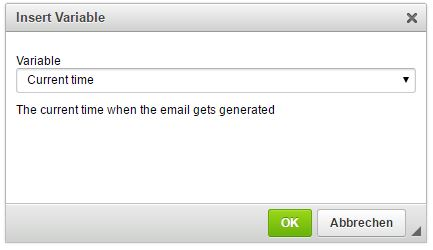
\includegraphics[scale=0.85]{ckeditor-dialog-insert-variable}
\caption{\emph{CKEditor} Dialog für die Variablenauswahl}
\label{fig:ckeditor-dialog-insert-variable}
\end{figure}
\ \newline
Die Abbildung \ref{fig:ckeditor-example-template} zeigt eine Vorlage innerhalb des \emph{CKEditors}, wobei die eingefügten Variablen besonders hervorgehoben werden. Die Bezeichnung  der Variable stellt den Namen für den \emph{HTML-Tag} bereit und die Beschreibung dessen Titel. Die eingefügten \emph{HTML-Tags} dürfen nicht verändert werden, daher ist das \emph{Drag} und \emph{Drop} und das Selektieren des eingefügten \emph{HTML-Tags} nicht erlaubt, da dadurch der eingefügte \emph{HTML-Tag} zerstört werden könnte und die Variablen nicht mehr gefunden werden können.
\begin{figure}[h]
\centering
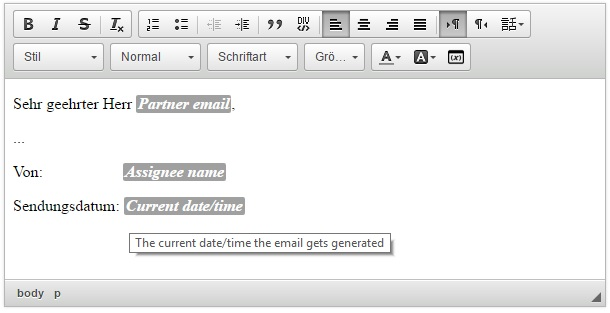
\includegraphics[scale=0.85]{ckeditor-example-template}
\caption{Beispiel einer Vorlage im \emph{CKEditor}}
\label{fig:ckeditor-example-template}
\end{figure}

\subsection{Die Implementierungen für \emph{CDI}}
\label{sec:sub-impl-integartion-cdi}
Dieser Abschnitt behandelt die Implementierungen für die Integration in eine \emph{CDI}-Umgebung, wie in Abschnitt \ref{sec:sub-template-management-cdi} beschrieben. Die Variablen werden über eine \emph{CDI}-Erweiterung gefunden und registriert und es werden die folgenden aufgelisteten Ressourcen kontextabhängig über einen implementierten \emph{CDI}-Erzeuger zur Verfügung gestellt: 
\begin{itemize}
 \item Das Objekt der Schnittstelle \emph{VariableConfiguration} 
 \newline
 ist das Objekt, dass die registrierten Variablen verwaltet.
 \item Die Objekte der Schnittstelle \emph{TemplateDataJsonBuilder}
 \newline
 sind Objekte, mit denen das \emph{JSON}-Datenobjekt für eine Vorlage und eine spezifische \emph{Template-Engine} erstellt werden kann.
 \item Die Objekte der Schnittstelle \emph{TemplateProcessor}
 \newline
 sind Objekte, mit denen Variablen in Vorlagen verwaltet werden können.
 \item Das Objekt der Klasse \emph{CdiTemplateUtil}
 \newline
 ist das Objekt mit dem die registrierten Variablen, die Objekte der Schnittstelle \emph{VariableContract} sind, in Objekte der Klasse \emph{VariableJson} konvertieren kann, wobei die Bezeichnung und die Beschreibung sprachspezifisch ermittelt werden.
\end{itemize}

\subsubsection{Die Vorlagenmanagement \emph{CDI}-Erweiterung}
Die implementierte \emph{CDI}-Erweiterung \emph{TemplateCdiExtension} findet beim Start der \emph{CDI}-Erweiterung die verfügbaren Variablen und hält die Variablen über die Lebensdauer der \emph{CDI}-Umgebung persistent. Eine \emph{CDI}-Erweiterung für eine muss folgende Voraussetzungen erfüllen, um geladen und verwendet werden zu können. 
\begin{enumerate}
	\item Sie muss die Schnittstelle \emph{javax.enterprise.inject.spi.Extension} implementieren,
	\item in einer Datei namens \emph{javax.enterprise.inject.spi.Extension}, die im Verzeichnis \emph{META-INF/services} liegen muss, mit ihren voll qualifizierten Namen registriert werden und
	\item das Artefakt, dass die \emph{CDI}-Erweiterung enthält muss eine Datei namens \emph{beans.xml} im Verzeichnis \emph{META-INF} enthalten.
\end{enumerate}
\ \newline
Die \emph{CDI}-Erweiterung wird beim Start der \emph{CDI}-Umgebung über den Mechanismus \emph{Service-Provider-Interface (SPI)} geladen und ein Objekt der Klasse der \emph{CDI}-Erweiterung erstellt. Dann kann das Objekt der \emph{CDI}-Erweiterung auf Ereignisse des Lebenszyklus der \emph{CDI}-Umgebung reagieren, in dem die \emph{CDI}-Erweiterung Beobachtermethoden für die einzelnen Ereignisse implementiert wie z.B.:
\begin{itemize}
	\item\emph{BeforeBeanDiscovery}
	\newline
	ist das Ereignis, das einmalig beim Start der \emph{CDI}-Umgebung aufgerufen wird bevor Typen, \emph{Beans} oder Injektionspunkte gesucht werden.
	\item\emph{ProcessAnnotatedType}
	\newline
	ist das Ereignis, das für jeden gefundenen injizierbaren Typ aufgerufen wird.
	\item\emph{AfterBeanDiscovery} 
	\newline
	ist das Ereignis, das einmalig Aufgerufen wird, wenn alle Typen, \emph{Beans} und Injektionspunkte gefunden und behandelt wurden.
\end{itemize}
\ \newline
Das erstellte Objekt der \emph{CDI}-Erweiterung ist an sich kein \emph{CDI-Bean}, da das Objekt der \emph{CDI}-Erweiterung bereits existiert bevor die \emph{CDI}-Umgebung vollständig gestartet wurde, ist aber trotzdem in andere \emph{CDI-Beans} injizierbar. Alle anderen \emph{CDI-Beans} können erst nachdem erfolgreichen Start der \emph{CDI}-Erweiterung injiziert werden.
\newline
\newline
Der Quelltext aus Abbildung \ref{prog:templateCdiExtension} ist ein Auszug aus der implementierten \emph{CDI}-Erweiterung \emph{TemplateCdiExtension} und zeigt die Beobachtermethoden, die auf Lebenszyklus Ereignisse der \emph{CDI}-Umgebung reagieren. Die  \emph{CDI}-Erweiterung \emph{TemplateCdiExtension} findet die Typen
\begin{itemize}
	\item alle implementierten Typen der Schnittstelle \emph{VariableContract}, die mit der Annotation \emph{CdiVariableContract} annotiert sind und
	\item alle implementierten Typen der Schnittstelle \emph{VariableResolverFactory}, die mit der Annotation \emph{CdiVariableResolverFactory} annotiert sind.
\end{itemize}
\ \newline
Die gefunden Typen werden in der \emph{CDI}-Erweiterung registriert und über die Lebensdauer der \emph{CDI}-Umgebung verwaltet. Bezüglich der Typen der Schnittstelle \emph{VariableContract} sei angemerkt, dass zur Zeit nur implementierte Typen vom Typ \emph{Enum} gefunden werden können. Alle Typen der Schnittstelle \emph{VariableContract}, die nicht vom Typ \emph{Enum} sind verursachen einen schweren Fehler und verhindern einen erfolgreichen Start der \emph{CDI}-Umgebung. Die Variablen könnten auch über implementierte Klassen der Schnittstelle \emph{VariableContract} implementiert werden und bei ihrer Verwendung dynamisch aus der \emph{CDI}-Umgebung geholt werden, was zur Zeit nicht benötigt wird.
\newline
\newline
Eine \emph{CDI}-Erweiterung ist eine injizierbare Ressource, die in jedes \emph{CDI-Bean} injiziert werden könnte, obwohl nur das Variablenmanagement sich das Objekt der \emph{CDI}-Erweiterung injizieren sollte. Es kann nicht verhindert werden, dass sich andere \emph{CDI-Beans} das Objekt der \emph{CDI}-Erweiterung injizieren lassen, da eine \emph{CDI}-Erweiterung öffentlich deklariert werden muss.

\begin{program}[h]
\caption{Auszug aus der \emph{CDI}-Erweiterung \emph{TemplateCdiExtension}}
\label{prog:templateCdiExtension}
\begin{JavaCode}
public class TemplateCdiExtension implements Extension {

    private TemplateConfiguration templateConfig;
    private Map<Class<? extends VariableContract>, 
                Class<VariableResolverFactory>>  
            variableResolverFactoryMap;

    void beforeBeanDiscovery(@Observes BeforeBeanDiscovery bbd) { ... }

    <T> void processCdiVariableContracts
             (@Observes @WithAnnotations({BaseName.class, 
                                          CdiVariableContract.class}) 
             ProcessAnnotatedType<T> pat) { ... }

    <T> void processVariableResolverFactoryFactories
        (@Observes @WithAnnotations(CdiVariableResolverFactory.class) 
        ProcessAnnotatedType<T> pat) { ... }
}
\end{JavaCode}
\end{program}
\ \newpage
\begin{itemize}
	\item\emph{beforeBeanDiscovery} 
	\newline
	ist die Beobachtermethode, die alle Objekte erstellt, die die gefundenen Typen über die Lebensdauer der \emph{CDI}-Umgebung verwalten.
	\item\emph{processCdiVariableContracts} 
	\newline
	ist die Beobachtermethode, die die gefundenen Typen der Schnittstelle \emph{VariableContract} behandelt.
	\item\emph{processVariableResolverFactoryFactories} 
	\newline
	ist die Beobachtermethode, die die gefundenen Typen der Schnittstelle \emph{VariableResolverFactory} behandelt.
\end{itemize}

\subsubsection{Der Vorlagenmanagement \emph{CDI}-Erzeuger}
Der implementierte \emph{CDI}-Erzeuger \emph{TemplateResourceProducer} produziert die kontextabhängigen Ressourcen des Vorlagenmanagements. Die Klasse \emph{TemplateResourceProducer} ist die einzige Klasse, in die das Objekt der \emph{CDI}-Erweiterung \emph{TemplateCdiExtension} injiziert wird. Im Kapitel \ref{cha:Lösungskonzept} wurde vorgegeben, dass mehrere \emph{Template-Engines} unterstützt werden müssen, daher wurde die Annotation \emph{@FreemarkerTemplate} eingeführt, die einen Injektionspunkt für die \emph{Template-Engine Freemarker} qualifiziert. In einer \emph{CDI}-Umgebung wird ein Qualifizierer benötigt, wenn für eine Schnittstelle mehrere Implementierungen zur Verfügung stehen, da ansonsten nicht entschieden werden kann welche Implementierung verwendet werden soll. Im Fall, dass es mehrere Implementierungen für eine Schnittstelle gibt, wird die Ausnahme \emph{AmbiguousResolutionException} geworfen und die \emph{CDI}-Umgebung kann nicht gestartet werden. 
\newline
\newline
Es wurden jeweils eine Erzeugermethode für den Qualifizierer \emph{@Default} und den Qualifizierer \emph{@FreemarkerTemplate} implementiert, womit nicht qualifizierte sowie qualifizierte Injektionspunkte versorgt werden können. Für die Erzeugermethode für den Qualifizierer \emph{@Default} wird die Implementierung für den Qualifizierer \emph{FreemarkerTemplate} verwendet, wodurch diese Implementierung als die Standardimplementierungen fungiert. Damit setzt man sich jedoch der Gefahr aus, dass die produzierte Standardimplementierung nicht die gewollte Implementierung ist, daher ist Vorsicht geboten, wenn diese Verhalten geändert werden sollte. 
\newline
\newline
Der Quelltext aus Abbildung \ref{prog:templateResourceProducer} ist ein Auszug aus der Klasse \emph{TemplateResourceProducer} und zeigt einige der implementierten Erzeugermethoden. 
\begin{program}[h]
\caption{Die Klasse \emph{TemplateResourceProducer}}
\label{prog:templateResourceProducer}
\begin{JavaCode}
@ApplicationScoped
public class TemplateResourceProducer implements Serializable {
    @Produces
    @ApplicationScoped
    @Default
    public VariableConfiguration produceConfiguration() {
        return extension.getVariableConfiguration();
    }
    
    @Produces
    @Dependent
    @Default
    public TemplateDataJsonBuilder produceDefaultTemplateBuilder
          (final @Default VariableResolverFactoryProvider factory) {
        return produceFreeMarkerTemplateBuilder(factory);
    }

    @Produces
    @Dependent
    @FreemarkerTemplate
    public TemplateDataJsonBuilder produceFreeMarkerTemplateBuilder
           (final @Default VariableResolverFactoryProvider factory) {
        return new FreemarkerTemplateDataJsonBuilder()
                      .withWeakMode()
                      .withVariableResolverFactoryProvider(factory);
    }
}
\end{JavaCode}
\end{program}
\ \newline
Diese beiden Methoden \emph{produceDefaultTemplateBuilder} und \emph{produceFreeMarkerTemplateBuilder} produzieren Objekte der Schnittstelle \emph{TemplateDataJsonBuilder} für den sogenannten Pseudo-\emph{Scope (@Dependent)}, wobei für jeden Injektionspunkt ein neues Objekt erstellt wird. Der Lebenszyklus von \emph{CDI-Beans} im Pseudo-\emph{Scope} wird nicht von der \emph{CDI}-Umgebung verwaltet und die Lebensdauer eines \emph{CDI-Bean} im Pseudo-\emph{Scope} ist gebunden and das \emph{CDI-Bean}, das sich das Pseudo-\emph{Scoped} \emph{CDI-Bean} injiziert hat. Die Erzeugermethoden \emph{produceDefaultTemplateBuilder} und \emph{produceFreeMarkerTemplateBuilder} lassen sich als Argument ein Objekt der Schnittstelle \emph{VariableResolverFactoryProvider} injizieren, dessen Geltungsbereich für diese Methoden nicht bekannt ist.
\newline
\newline
Die Methode \emph{produceConfiguration} produziert ein Objekt der Schnittstelle  \emph{VariableConfiguration}, das die registrierten Variablen enthält und von der \emph{CDI}-Erweiterung bereitgestellt wird. Nachdem die Schnittstelle  \emph{VariableConfiguration} nur lesenden Zugriff erlaubt, wird dieses Objekt für den Gültigkeitsbereich der Anwendung produziert, also einmalig für die gesamte Lebensdauer der \emph{CDI}-Umgebung.
\newline
\newline
Alle injizierbaren Objekte werden erst beim ersten Zugriff auf eine ihrer öffentlichen Methoden erzeugt und im korrespondierenden Geltungsbereich registriert. Sollte ein injizierbares Objekt niemals verwendet werden, so wird es auch niemals erzeugt. Dieses Verhalten ist möglich, da alle Injektionspunkte von \emph{Proxies} verwaltet werden, die beim Starten der \emph{CDI}-Umgebung in die Injektionspunkte injiziert werden und ein abgeleiteter Typ des injizierten Typs sind. Bei einem Zugriff auf eine öffentliche Methode des injizierten Objekts, wird das korrespondierende Objekt aus den aktuellen Geltungsbereich geholt und der Aufruf an dieses Objekt weiter delegiert.  

\subsubsection{Die Vorlagenmanagement \emph{CDI}-Hilfsklasse}
Die Klasse \emph{CdiTemplateUtil} aus dem Quelltext aus Abbildung \ref{prog:cdiTemplateUtil} wurde implementiert, um ein injizierbares \emph{CDI-Bean} zur Verfügung zu stellen, das Hilfsmethoden für die Konvertierung der Variablen von Objekten der Schnittstelle \emph{VariableContract} in Objekte der Klasse \emph{VariableJson} und visa versa zur Verfügung stellt. Diese Implementierung hält keinen Status, daher kann dieses \emph{CDI-Bean} in den Geltungsbereich der Anwendung registriert werden. Die Verwendung des Objekts der Klasse \emph{CdiTemplateUtil} ist \emph{Thread-Safe}
\begin{itemize}
	\item da kein Status in diesem Objekt gehalten wird und
	\item das verwendete Objekt der Klasse \emph{TemplateConfiguration} nur lesenden Zugriff erlaubt.
\end{itemize}
\ \newline
Die Annotation \emph{@Typed(CdiTemplateUtil.class)} bewirkt dass dieses \emph{CDI-Bean} nur über den Typ \emph{CdiTemplateUtil} injizierbar ist. Mit der Annotation \emph{@Typed} kann man einschränken, über welche Typen ein \emph{CDI-Bean} injizierbar ist, was hilfreich ist, wenn die Klasse eines \emph{CDI-Beans} mehrere Schnittstellen implementiert.

\begin{program}[h]
\caption{Die Klasse \emph{CdiTemplateUtil}}
\label{prog:cdiTemplateUtil}
\begin{JavaCode}
@ApplicationScoped
@Typed(CdiTemplateUtil.class)
public class CdiTemplateUtil implements Serializable {

    @Inject
    private VariableConfiguration config;

    public List<VariableJson> convertContractToJsonModel
    						  (final Locale locale) { }

    public List<VariableJson> convertContractToJsonModel
    		(final Collection<VariableContract> contracts,
             final Locale locale) { }

    public VariableJson convertContractToJsonModel
           (final VariableContract contract,
            final Locale locale) { }
	
    public List<VariableContract> convertJsonModelToContract
    							 (final Collection<VariableJson> jsonModels) { }

    public VariableContract convertJsonModelToContract
                            (final VariableJson jsonModel) { }
}
\end{JavaCode}
\end{program}

\subsection{Die Implementierungen für \emph{JSF}}
\label{sec:sub-impl-integartion-jsf}
Dieser Abschnitt beschäftigt sich mit der Implementierung der Integration des Variablenmanagements in die \emph{View}-Technologie \emph{JSF}, wie im Abschnitt \ref{sec-sub-specification-jsf} vorgegeben. Es werden der implementierte \emph{FacesConverter} und die \emph{CKEditor}-Integration in \emph{JSF} behandelt.

\subsubsection{Der Vorlagen \emph{FacesConverter}}
Ein \emph{FacesConverter} ist eine Klasse für die Konvertierung in \emph{JSF}, welche die Schnittstelle \emph{javax.faces.convert.Converter} implementiert, wobei diese Schnittstelle die folgenden beiden Methoden definiert.
\begin{itemize}
	\item\emph{getAsObject}
	\newline
	ist die Methode, die den Wert des Parameters, in Form von einer Zeichenkette, in das korrespondierende \emph{Java}-Objekt konvertiert und
	\item\emph{getAsString}
	\newline
	ist die Methode, die ein \emph{Java}-Objekt in eine Zeichenkette konvertiert.
\end{itemize}
\ \newline
Ein \emph{FacesConverter} wird im \emph{JSF-Framework} über die Annotation \emph{FacesConverter("converterName")} oder einen Eintrag in der der Konfigurationsdatei \emph{faces-config.xml} registriert. Einer \emph{JSF}-Komponente kann in \emph{XHTML} über das Attribut \emph{converter} ein Konverter, entweder 
\begin{itemize}
	\item über dessen registrierten Namen oder 
	\item durch Parameterbindung auf ein Objekt des Konverters, zugewiesen werden.
\end{itemize}
Die gemeinsame Logik wurde in einer abstrakten Klasse \emph{AbstractTemplateConverter} zusammengefasst, da sich lediglich die konkrete Implementierungen der Schnittstelle \emph{TemplateProcessor} für die verschiedenen \emph{Template-Enginges} unterscheidet. Da keine Injektion in \emph{JSF}-Artefakte \emph{JSF 2.2} wie z.B.
\begin{itemize}
	\item\emph{FacesConverter},
	\item\emph{FacesValidator} order
	\item\emph{Component}
\end{itemize}
möglich ist, wurde die abstrakte Klasse \emph{AbstractTemplateConverter} implementiert und eine konkrete Implementierung für die \emph{Template-Engine Freemarker}. Ab \emph{JSF 2.3} wird in \emph{JSF}-Artefakten Injektion zur Verfügung stehen. Die Implementierung der Klasse \emph{FreemarkerTemplateConverter}, die von der Klasse \emph{AbstractTemplateConverter} ableitet, setzt über den Konstruktor statisch den zu verwendenden Qualifizierer, mit dem über die Hilfsklasse \emph{BeanProvider} der Bibliothek \emph{DeltaSpike} dynamisch die benötigten \emph{CDI-Beans} von der \emph{CDI}-Umgebung geholt werden. Beim Erstellen eines Objekts der Klasse \emph{FreemarkerTemplateConverter} muss ein Objekt der Klasse \emph{java.util.Locale} übergeben werden, damit die Bezeichnung und die Beschreibung einer Variable in einer Vorlage sprachspezifisch konvertiert werden kann. Die definierte Sprache sollte die Sprache sein, für die die Vorlage erstellt wurde.

\begin{program}[h]
\caption{Die Klasse \emph{FreemarkerTemplateConverter}}
\label{prog:freemarkerTemplateConverter}
\begin{JavaCode}
public class FreemarkerTemplateConverter 
                          extends AbstractTemplateConverter {

    public FreemarkerTemplateConverter(final Locale locale) {
        super(new FreemarkerTemplateLiteral(), locale);
    }
}
\end{JavaCode}
\end{program}
\ 
\newline
Die abstrakte Klasse \emph{AbstractTemplateConverter} definiert reguläre Ausdrücke, um die Variablen in einer Vorlage in Form von \emph{HTML-Tags} zu finden und zu konvertieren.
\begin{JavaCode}[numbers=none]
String tagRegex = "(<span[^>]*class=\"variable\"[^>]*>[^<]*</span>)";
String idRegex  = "data-variable-id=\"(\\S+)\"";
\end{JavaCode}
\ \begin{itemize}
	\item\emph{tagRegex}
	\newline
	ist der reguläre Ausdruck, um die Variablen in ihrer \emph{HTML}-Repräsentation in einer Vorlage zu finden.
	\item\emph{idRegex}
	\newline
	ist der reguläre Ausdruck, um die \emph{Id} einer Variable, aus deren \emph{HTML}-Repräsentation zu bekommen und wird auf den gefundenen \emph{HTML-Tag} einer Variable angewendet, die mit dem regulären Ausdruck \emph{tagRegex} gefunden wurde.
\end{itemize}
\ \newline
Die abstrakte Klasse \emph{AbstractTemplateConverter} definiert auch eine Vorlage in Form einer Zeichenkette, mit der die Variablen in ihre \emph{HTML-Tag}-Repräsentation konvertiert werden können, wobei diese Vorlage unabhängig von der verwendeten \emph{Template-Engine} ist.
\begin{JavaCode}
String template = "<span class=\"variable\" contentEditable=\"false\" "
                + "data-variable-id=\"{0}\" title=\"{1}\">{2}</span>";
\end{JavaCode}
Die Vorlage \emph{template} wird mit \emph{java.text.MessageFormat(String, Object...)} verarbeitet, wobei der Formalparameter \emph{Object...} eine variable Argumentliste ist, über welche die dynamischen Werte für die Vorlage bereitgestellt werden können. 

\subsubsection{Die \emph{Primefaces-Extension} für den \emph{CKEditor}}
Der \emph{Editor CKEditor} ist eine \emph{JavaScript} basierte Anwendung, die nur am \emph{Browser} der BenutzerInnen läuft. Es wird eine Integration in \emph{JSF} benötigt, damit man
\begin{itemize}
	\item auf \emph{AJAX-Events} reagieren kann,
	\item\emph{FacesConverter} verwenden kann und
	\item Parameterbindungen definieren kann.
\end{itemize}
\ \newline
Es ist nicht trivial ist eine vollwertige \emph{JSF}-Komponente zu implementieren und das Implementieren einer solchen Komponente nimmt auch viel Zeit in Anspruch. Daher wurde auf die Implementierung von \emph{PrimeFaces-Extensions} zurückgegriffen, die bereits eine vollwertige \emph{JSF}-Integration in Form einer \emph{JSF}-Komponente für den \emph{CKEditor} bereitstellt.
\newline
\newline
Die Ressourcen für den \emph{CKEDitor} bewegen sich in der Größenordnung von 1,5 \emph{Megabyte}, daher werden die Ressourcen in einem separaten Artefakt zur Verfügung gestellt. Man kann auch eine eigene Implementierung des \emph{CKEditors} zur Verfügung stellen, sofern diese Implementierung in derselben Version vorhanden ist, wie von \emph{PrimeFaces-Extensions} unterstützt wird. Der \emph{CKEditor} ist ein sehr umfangreicher \emph{Editor}, den man sich auch seinen Wünschen entsprechend über die Webseite \url{http://ckeditor.com/builder} selbst zusammenstellen kann.
\newline
\newline
Der Quelltest aus Abbildung \ref{prog:example-ckeditor-xhtml} zeigt die Verwendung der \emph{JSF}-Komponente für den \emph{CKEditor}.
\begin{program}[h]
\caption{Verwendung der \emph{JSF}-Komponente für den \emph{CKEditor}}
\label{prog:example-ckeditor-xhtml}
\begin{HtmlCode}
<pe:ckEditor id="view_id"
             wdgetVar="pfEditor"
             value="#{model.content}"
             converter="#{viewBean.converter}" 
             contentsCss="resources/css/myStyle.css"
             customConfig="./ckeditor-config.js">
</pe:ckEditor>
\end{HtmlCode}
\end{program}
\ \begin{itemize}
	\item\emph{id} 
	\newline
	ist das Attribut, um die eindeutige \emph{Id} innerhalb des Namensraums, in dem sich die Komponente befindet, zu definieren.
	\item\emph{widgetVar}
	\newline
	ist das Attribut, um einen global eindeutigen Namen des \emph{JavaScript}-Objekts \emph{Widget} zu definieren, das den Zugriff auf den \emph{CKEditor} innerhalb von \emph{JavaScript} ermöglicht.
	\item\emph{value}
	\newline
	ist das Attribut, um die Parameterbindung des Inhalts des \emph{CKEditors} zu einem \emph{Java}-Model zu definieren.
	\item\emph{converter}
	\newline
	ist das Attribut, um den zu verwendeten Konverter über seinen eindeutigen Namen oder einer Parameterbindung zu setzen.
	\item\emph{contentCss}
	\newline
	ist das Attribut, um eine eigene \emph{CSS}-Datei für den Inhalt der Vorlage zu definieren. Die Vorlage wird innerhalb des \emph{Editors} als eigenständige \emph{HMTL}-Datei behandelt, das in einer \emph{HTML-IFrame}-Komponente gehalten wird.
	\item\emph{customConfig}
	\newline
	ist das Attribut, um die eine eigene Konfiguration des \emph{Editors} in Form von einer \emph{JavaScript}-Datei zu definieren. 
\end{itemize}

\section{Die Vorlagenmanagement Beispielanwendung}
Dieser Abschnitt beschäftigt sich mit der implementierten Beispielanwendung für das Vorlagenmanagement, welche die Verwendung des Vorlagenmanagement im Bezug auf 
\begin{itemize}
	\item die Verwendung in der Geschäftslogik,
	\item die Verwendung über eine Webseite und
	\item die Verwendung zum Erstellen einer \emph{E-Mail} aufzeigen soll. 
\end{itemize}

\subsection{Die Verwendung über eine \emph{Web}-Oberfläche}
Die Abbildung \ref{fig:demo_web_app_empty_view_part_1} zeigt die Weboberfläche, die für die Beispielanwendung implementiert wurde. Über dieses Formular können die Voralgen sprachspezifisch verwaltet werden.
\ \begin{figure}[h]
\centering
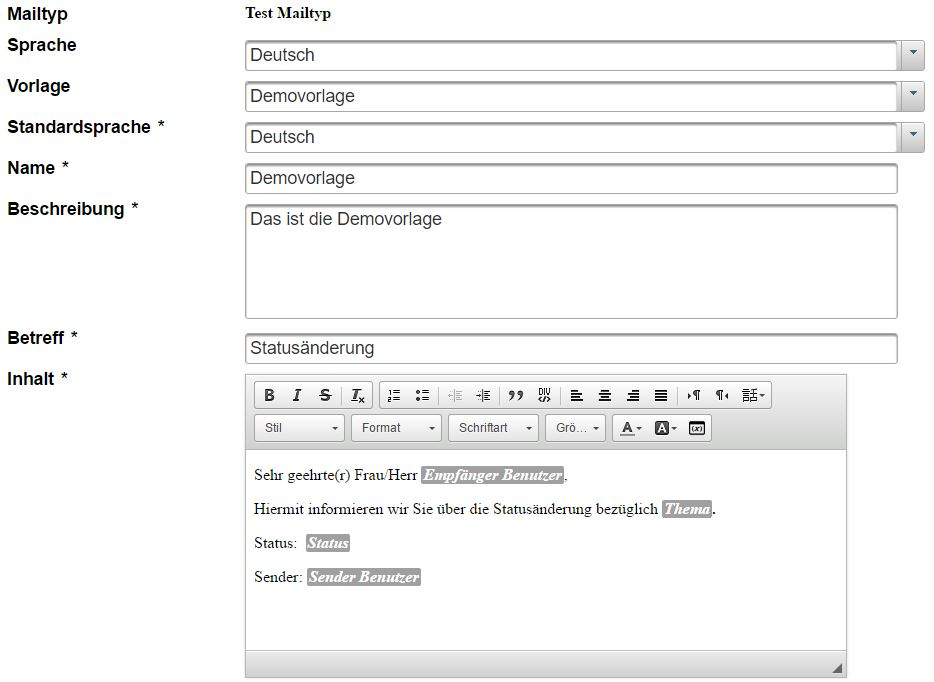
\includegraphics[scale=0.5]{demo_web_app_empty_view_part_1}
\caption{Formular für die Verwaltung der Vorlagen}
\label{fig:demo_web_app_empty_view_part_1}
\end{figure}
\ \newline
Die Abbildung \ref{fig:demo_web_app_empty_view_part_2} zeigt, den Teil der Webseite, der die relevanten Daten einer Vorlage anzeigt.
\begin{itemize}
	\item\emph{Decorator Template} ist die \emph{Freemarker}-Voralge, die von jeder Vorlage dekoriert wird.
	\item\emph{User Template} ist die Vorlage, die von einem BenutzerIn erstellt wurde.
	\item\emph{Template JSON Data} ist die \emph{JSON}-Zeichenkette, die erstellt wird, wenn die Daten für eine Vorlage serialisiert werden.
	\item\emph{Parsed Template} ist die Vorlage, in der die Variablen durch die serialisierten Werte ersetzt wurden.
	\item\emph{Template Metadata} sind die Metadaten der Vorlage, wie z.B. die Anzahl der enthalten Variablen.
\end{itemize}
\begin{figure}[h]
\centering
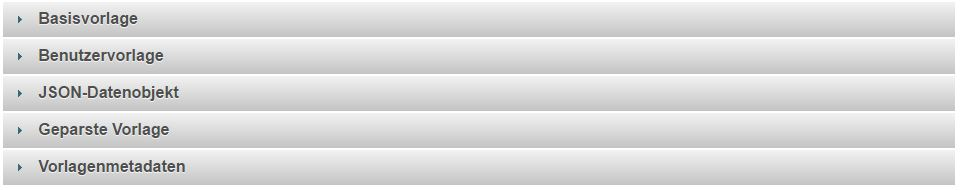
\includegraphics[scale=0.5]{demo_web_app_empty_view_part_2}
\caption{Anzeige der aller relevanten Daten einer Vorlage}
\label{fig:demo_web_app_empty_view_part_2}
\end{figure}

\subsubsection{Die Dekoriervorlage}
Der Quelltext aus Abbildung \ref{prog:demo_web_app_data_decorator} zeigt die dekorierbare \emph{Freemarker}-Vorlage, die alle Vorlagen dekorieren. Sie stellt den \emph{HTML-Body} zur Verfügung, da die Benutzervoralgen nur den Inhalt innerhalb des \emph{HTML-Tags Body} bereitstellen.
\begin{program}[h]
\caption{Die dekorierbare \emph{Freemarker}-Vorlage}
\label{prog:demo_web_app_data_decorator}
\begin{HtmlCode}
<#-- This macro is used to add decorated template dynamically -->
<#macro includeMacro templateName>
    <#include "${templateName}" encoding="UTF-8">
</#macro>
<!DOCTYPE html>
<html lang="en">
<meta http-equiv="Content-Type" content="text/html; charset=utf-8">
<body>
<div style="margin: 10px;">
    <div style="padding: 5px;">
    <@includeMacro templateName="${TEMPLATE_NAME}" />
    </div>
    <div style="padding: 5px;">
    <@includeMacro templateName="${FOOTER_TEMPLATE}" />
    </div>
</div>
</body>
</html>
\end{HtmlCode}
\end{program}
\ \newpage
%$ : otherwise everything afterwards is marked green

\subsubsection{Die Benutzervorlage}
Der Quelltext aus Abbildung \ref{prog:demo_web_app_data_template} zeigt die \emph{Freemarker}-Vorlage, die von der BenutzerInnen erstellt wird. Die Vorlage enthält zwar \emph{HTML-Markup}, aber nur den Inhalt unterhalb des \emph{HTML-Tags Body}. Sie stellt daher kein vollständiges \emph{HTML}-Dokument zur Verfügung, wofür die Dekoriervorlage aus Abbildung \ref{prog:demo_web_app_data_decorator} implementiert wurde.
\begin{program}[h]
\caption{Die BenutzerIn \emph{Freemarker}-Vorlage}
\label{prog:demo_web_app_data_template}
\begin{HtmlCode}
<p>Sehr geehrte(r) Frau/Herr&nbsp;
${(cc.module.di["RECIPIENT_USER"])!("variable: 'RECIPIENT_USER' not found")}
,</p>

<p>Hiermit informieren wir Sie &uuml;ber die Status&auml;nderung 
bez&uuml;glich&nbsp;
<strong>
${(cc.module.di["TOPIC"])!("variable: 'TOPIC' not found")}.
</strong>
</p>

<p>Status: &nbsp;
${(cc.module.di["STATUS"])!("variable: 'STATUS' not found")}
</p>

<p>Sender:&nbsp;
${(cc.module.di["SENDER_USER"])!("variable: 'SENDER_USER' not found")}
</p>

<p>&nbsp;</p>
\end{HtmlCode}
\end{program}
\ \newpage

\subsubsection{Das serialisierte \emph{JSON}-Datenobjekt}
Der Quelltext aus Abbildung \ref{prog:demo_web_app_data_json} zeigt die serialisierte \emph{JSON}-Zeichenkette, die beim Erstellen einer \emph{E-Mail} erstellt wird und in der Datenbank persistent gehalten wird. Mit diesen Daten kann eine \emph{E-Mail} auf Basis dieser Vorlage jederzeit wiederhergestellt werden.

\begin{program}[h]
\caption{Das \emph{JSON}-Datenobjekt}
\label{prog:demo_web_app_data_json}
\begin{JsCode}
{
  "@type" : "template-data-json",
  "unknownProperties" : { },
  "template_metadata" : {
    "@type" : "template-metadata-json",
    "unknownProperties" : { },
    "id" : 1,
    "version" : 1,
    "locale" : "de",
    "zoneId" : "Europe/London",
    "variableCount" : 4
  },
  "data" : {
    "cc" : {
      "module" : {
        "di" : {
          "STATUS" : "Inatkiv",
          "RECIPIENT_USER" : "Hugo Maier",
          "TOPIC" : "BenutzerIn Status geändert",
          "SENDER_USER" : "Thomas Herzog"
        }
      }
    }
  }
}
\end{JsCode}
\end{program}
\ \newpage

\subsubsection{Die geparste Benutzervorlage}
Der Quelltext aus Abbildung \ref{prog:demo_web_app_data_parsed_template} zeigt die geparste Vorlage. Die Variablen der Vorlage aus dem Quelltext aus Abbildung \ref{prog:demo_web_app_data_template} wurden durch den serialisierten Wert des \emph{JSON}-Datenobjekts aus dem Quelltext aus Abbildung \ref{prog:demo_web_app_data_json} ersetzt.

\begin{program}[h]
\caption{Das \emph{JSON}-Datenobjekt}
\label{prog:demo_web_app_data_parsed_template}
\begin{HtmlCode}
<!DOCTYPE html>
<html lang="en">
    <meta http-equiv="Content-Type" content="text/html; charset=utf-8">
<body>
<div style="margin: 10px;">
    <div style="padding: 5px;">
        <p>Sehr geehrte(r) Frau/Herr&nbsp;Hugo Maier,</p>

        <p>
            Hiermit informieren wir Sie &uuml;ber die 
            Status&auml;nderung bez&uuml;glich&nbsp;
            <strong>BenutzerIn Status geändert.</strong>
        </p>

        <p>Status: &nbsp;Inatkiv</p>

        <p>Sender:&nbsp;Thomas Herzog</p>

        <p>&nbsp;</p>
    </div>
    <div style="padding: 5px;">
    </div>
</div>
</body>
</html>
\end{HtmlCode}
\end{program}
\ \newpage

\subsubsection{Die Vorlagenmetadaten}
Der folgende Text zeigt die Zeichenkette, welchen die in Abschnitt \ref{sec:abstractTemplateMetadata} vorgestellte Klasse \emph{AbstractTemplateMetadata} produziert. Diese Ausgabe ist nur für Entwicklungszwecke interessant und zeigt die aktuellen Metadaten der Vorlage aus dem Quelltext aus Abbildung \ref{prog:demo_web_app_data_template}.

\begingroup
    \fontsize{9pt}{11pt}\selectfont
    \begin{verbatim}  
===============================================================
FreemarkerTemplateMetadata
===============================================================
id                  : 1
version             : 1
length              : 482
variables (valid)   : 4
contract  : com.clevercure.mailing.demo.logic.variable.TemplateVariable
id        : cc.module.di.SENDER_USER
name      : SENDER_USER
label-key : SENDER_USER
info-key  : SENDER_USER


contract  : com.clevercure.mailing.demo.logic.variable.TemplateVariable
id        : cc.module.di.STATUS
name      : STATUS
label-key : STATUS
info-key  : STATUS


contract  : com.clevercure.mailing.demo.logic.variable.TemplateVariable
id        : cc.module.di.RECIPIENT_USER
name      : RECIPIENT_USER
label-key : RECIPIENT_USER
info-key  : RECIPIENT_USER


contract  : com.clevercure.mailing.demo.logic.variable.TemplateVariable
id        : cc.module.di.TOPIC
name      : TOPIC
label-key : TOPIC
info-key  : TOPIC

variables (invalid) : 0
    \end{verbatim}  
\endgroup
\newpage

\subsection{Die Verwendung in einer Geschäftslogik}
Der Quelltext aus Abbildung \ref{prog:emailServiceCdiEventImpl} zeigt die implementierte Klasse \emph{EmailServiceCdiEventImpl} der Schnittstelle \emph{EmailService}, die spezifiziert wie über eine Geschäftslogik \emph{E-Mails} erstellt werden können. Die Implementierung \emph{EmailServiceCdiEventImpl} verwendet die implementierte Klasse \emph{CreateEmailsEvent}, die ein \emph{Event}-Objekt darstellt, das über den \emph{CDI-Event-Bus} verarbeitet wird. Es wir ein Objekt der Schnittstelle \emph{javax.enterprise.Event} injiziert, das mit dem \emph{Event}-Objekt typisiert ist. Die Injektionspunkte der \emph{Events} wurden qualifiziert, damit verschiedene Beobachtermethoden aufgerufen werden können.

\begin{program}[h]
\caption{Die Klasse \emph{EmailServiceCdiEventImpl}}
\label{prog:emailServiceCdiEventImpl}
\begin{JavaCode}
@RequestScoped
@Transactional(Transactional.TxType.SUPPORTS)
public class EmailServiceCdiEventImpl implements EmailService {
    @Inject
    @Immediate
    private Event<CreateEmailsEvent> createImmediateEvent;
    @Inject
    @AfterSuccess
    private Event<CreateEmailsEvent> createAfterSuccessEvent;

    @Override
    @Transactional(Transactional.TxType.REQUIRED)
    public void create(EmailDTO dto) {
        createImmediateEvent.fire(new CreateEmailsEvent(dto));
    }

    @Override
    @Transactional(Transactional.TxType.REQUIRED)
    public void create(List<EmailDTO> dtos) {
        createImmediateEvent.fire(new CreateEmailsEvent(dtos));
    }

    @Override
    public void createAfterSuccess(EmailDTO dto) {
        createAfterSuccessEvent.fire(new CreateEmailsEvent(dto));
    }

    @Override
    public void createAfterSuccess(List<EmailDTO> dtos) {
        createAfterSuccessEvent.fire(new CreateEmailsEvent(dtos));
    }
}
\end{JavaCode}
\end{program}
\ \newpage
Folgende Auflistung erklärt die implementierten Methoden der Klasse \emph{EmailServiceCdiEventImpl} der Schnittstelle \emph{EmailService}, über die von einer Geschäftslogik aus \emph{E-Mails} erstellt werden können.
\begin{itemize}
	\item\emph{create(EmailDTO dto)}
	\newline
	ist die Methode, mit der eine \emph{E-Mail} sofort erstellt werden kann, wobei beim Feuern des \emph{Events} die aktuelle Ausführung der Methode unterbrochen und synchron die Beobachtermethode aufgerufen wird.
	\item\emph{create(List<EmailDTO> dtos)}
	\newline
	ist die Methode, mit der mehrere \emph{E-Mails} sofort erstellt werden können. Das Verhalten ist gleich wie bei der Methode \emph{create(EmailDTO dto)}.
	\item\emph{createAfterSuccess(EmailDTO dto)}
	\newline
	ist die Methode, mit der eine \emph{E-Mail}, nach dem erfolgreichem Beenden einer Transaktion, erstellt werden kann, wobei die Beobachtermethode trotzdem noch in der Komplettierungsphase der Transaktion aufgerufen wird.
	\item\emph{createAfterSuccess(List<EmailDTO> dto)}
	\newline
	ist die Methode, mit der mehrere \emph{E-Mails}, nach dem erfolgreichem Beenden einer Transaktion, erstellt werden können. Das Verhalten ist gleich wie in der Methode \emph{createAfterSuccess(EmailDTO dto)}.
 werden kann.    
\end{itemize} 
\ \newline
Der Quelltext aus Abbildung \ref{prog:businessServiceImpl} zeigt die implementierte Klasse \emph{BusinessServiceImpl}, welche die Geschäftslogik simuliert, die über die Schnittstelle \emph{EmailService} \emph{E-Mails} erstellt. Die zu erstellende \emph{E-Mail} wird durch ein Objekt der Klasse \emph{EmailDTO} repräsentiert, welche alle benötigten Informationen für das Erstellen einer \emph{E-Mail} enthält. Das Objekt der Schnittstelle \emph{Emailservice} wird über Injektion von der \emph{CDI}-Umgebung bereitgestellt. Wie im Kapitel \ref{cha:Zielsetzung} vorgegeben dürfen die Anwendungen nicht wissen, wie \emph{E-Mails} erstellt werden, was über die Schnittstelle \emph{EmailService} realisiert wurde. Dieser Geschäftslogik ist die konkrete Implementierung der Schnittstelle \emph{EmailService} nicht bekannt und daher auch nicht dass die \emph{E-Mails} über \emph{CDI-Events} bzw. deren Beobachtermethoden erstellt werden.
\newline
\newline
Die \emph{E-Mails} werden innerhalb, der von der Klasse \emph{BusinessServiceImpl} geöffneten Transaktion, erstellt. Es ist nicht möglich eine Transaktion in einer Beobachtermethode zu öffnen, da die \emph{Events} immer in der Komplettierungsphase der geöffneten Transaktion behandelt werden und es keine Möglichkeit, dies zu umgehen.
\newpage
\begin{program}[h]
\caption{Die Klasse \emph{BusinessServiceImpl}}
\label{prog:businessServiceImpl}
\begin{JavaCode}
@RequestScoped
@Transactional(Transactional.TxType.REQUIRED)
public class BusinessServiceImpl implements BusinesService {
    @Inject
    private EmailService emailService;
    @Override
    public void doBusinessEmailImmediate() {
        emailService.create(createEmailDto());
    }

    @Override
    public void doBusinessEmailAfterSuccess() {
        emailService.createAfterSuccess(createEmailDto());
    }

    private EmailDTO createEmailDto() {
        final String email = "herzog.thomas8@gmail.com";
        final Long mailUserId = 1L;
        final List<Long> mailTypeIds = Collections.singletonList(1L);
        final Locale locale = Locale.US;
        final ZoneId zone = ZoneId.systemDefault();
        final Map<Object, Object> userData = 
        	new HashMap<Object, Object>() {{
                put(TemplateVariable.SENDER_USER, "Thomas Herzog");
                put(TemplateVariable.RECIPIENT_USER, "Hugo Maier");
                put(TemplateVariable.TOPIC, "User status changed");
                put(TemplateVariable.STATUS, "Inactive");
            }};
        return new EmailDTO(email, 
        					locale, 
        					zone, 
        					mailUserId, 
        					userData, 
        					mailTypeIds);
    }
}
\end{JavaCode}
\end{program}
\ \newline
Folgende Auflistung erklärt die Attribute, die beim Erstellen eines Objekts der Klasse \emph{EmailDto} angegeben werden müssen.
\begin{itemize}
	\item\emph{email}
	\newline
	ist die Zeichenkette, welche die \emph{E-Mail}-Adresse definiert.
	\item\emph{mailUserId}
	\newline
	ist die \emph{Id} des internen \emph{Mail}-Benutzers, welcher die \emph{E-Mail} auf der Datenbank erstellt.
	\item\emph{mailTypeIds}
	\newline
	ist die Menge von \emph{Ids}, welche die \emph{Mail}-Typen repräsentieren. Jedem \emph{Mail}-Typ ist eine Voralge zugeordnet.
	\item\emph{locale}
	\newline
	ist das Objekt der Klasse \emph{java.util.Locale}, das die Sprache definiert.
	\item\emph{zone} 
	\newline
	ist das Objekt der Klasse \emph{java.time.ZoneId}, das die Zone für die Datumsformatierung definiert.
	\item\emph{userData} 
	\newline
	ist der assoziative Behälter, der die Benutzerdaten enthält, die bei der Ermittlung der aktuellen Werte der Variablen verwendet werden können.
\end{itemize}